\documentclass[a4paper]{book}
\usepackage{a4wide}
\usepackage{makeidx}
\usepackage{fancyhdr}
\usepackage{graphicx}
\usepackage{multicol}
\usepackage{float}
\usepackage{textcomp}
\usepackage{alltt}
\usepackage{doxygen}
\makeindex
\setcounter{tocdepth}{1}
\renewcommand{\footrulewidth}{0.4pt}
\begin{document}
\begin{titlepage}
\vspace*{7cm}
\begin{center}
{\Large liburbi-cpp Reference Manual\\[1ex]\large 1.0 }\\
\vspace*{1cm}
{\large Generated by Doxygen 1.3.9.1}\\
\vspace*{0.5cm}
{\small Wed Sep 21 08:43:19 2005}\\
\end{center}
\end{titlepage}
\clearemptydoublepage
\pagenumbering{roman}
\tableofcontents
\clearemptydoublepage
\pagenumbering{arabic}
\chapter{liburbi-cpp Namespace Index}
\section{liburbi-cpp Namespace List}
Here is a list of all documented namespaces with brief descriptions:\begin{CompactList}
\item\contentsline{section}{{\bf urbi} (Namespace containing wrappers for platform-dependant functions )}{\pageref{namespaceurbi}}{}
\end{CompactList}

\chapter{liburbi-cpp Hierarchical Index}
\section{liburbi-cpp Class Hierarchy}
This inheritance list is sorted roughly, but not completely, alphabetically:\begin{CompactList}
\item \contentsline{section}{UAbstract\-Client}{\pageref{classUAbstractClient}}{}
\begin{CompactList}
\item \contentsline{section}{UClient}{\pageref{classUClient}}{}
\begin{CompactList}
\item \contentsline{section}{USync\-Client}{\pageref{classUSyncClient}}{}
\end{CompactList}
\end{CompactList}
\item \contentsline{section}{UBinary}{\pageref{classUBinary}}{}
\item \contentsline{section}{UImage}{\pageref{classUImage}}{}
\item \contentsline{section}{UMessage}{\pageref{classUMessage}}{}
\item \contentsline{section}{USound}{\pageref{classUSound}}{}
\end{CompactList}

\chapter{liburbi-cpp Class Index}
\section{liburbi-cpp Class List}
Here are the classes, structs, unions and interfaces with brief descriptions:\begin{CompactList}
\item\contentsline{section}{{\bf UAbstract\-Client} (Interface for an URBI wrapper object )}{\pageref{classUAbstractClient}}{}
\item\contentsline{section}{{\bf UBinary} (Class containing binary data sent by the server, that could not be furtehr interpreted )}{\pageref{classUBinary}}{}
\item\contentsline{section}{{\bf UClient} (Linux implementation of {\bf UAbstract\-Client}{\rm (p.\,\pageref{classUAbstractClient})} )}{\pageref{classUClient}}{}
\item\contentsline{section}{{\bf UImage} (Class encapsulating an image )}{\pageref{classUImage}}{}
\item\contentsline{section}{{\bf UMessage} (Class containing all informations related to an URBI message )}{\pageref{classUMessage}}{}
\item\contentsline{section}{{\bf USound} (Class encapsulating sound informations )}{\pageref{classUSound}}{}
\item\contentsline{section}{{\bf USync\-Client} ({\bf UClient}{\rm (p.\,\pageref{classUClient})} linux implementation with support for synchronous functions )}{\pageref{classUSyncClient}}{}
\end{CompactList}

\chapter{liburbi-cpp File Index}
\section{liburbi-cpp File List}
Here is a list of all documented files with brief descriptions:\begin{CompactList}
\item\contentsline{section}{{\bf uabstractclient.cpp} }{\pageref{uabstractclient_8cpp}}{}
\item\contentsline{section}{{\bf uabstractclient.h} }{\pageref{uabstractclient_8h}}{}
\item\contentsline{section}{{\bf uclient.cpp} }{\pageref{uclient_8cpp}}{}
\item\contentsline{section}{{\bf uclient.h} }{\pageref{uclient_8h}}{}
\item\contentsline{section}{{\bf usyncclient.cpp} }{\pageref{usyncclient_8cpp}}{}
\item\contentsline{section}{{\bf usyncclient.h} }{\pageref{usyncclient_8h}}{}
\end{CompactList}

\chapter{liburbi-cpp Namespace Documentation}
\section{urbi Namespace Reference}
\label{namespaceurbi}\index{urbi@{urbi}}
Namespace containing wrappers for platform-dependant functions.  


\subsection*{Functions}
\begin{CompactItemize}
\item 
void {\bf execute} (void)\label{namespaceurbi_a5}

\begin{CompactList}\small\item\em This function must be called at the last line of your main() function. \item\end{CompactList}\item 
void {\bf exit} (int code)\label{namespaceurbi_a6}

\begin{CompactList}\small\item\em This function will terminate your URBI program. \item\end{CompactList}\item 
{\bf UClient} \& {\bf connect} (const char $\ast$host)\label{namespaceurbi_a7}

\begin{CompactList}\small\item\em Creates a new {\bf UClient}{\rm (p.\,\pageref{classUClient})} object. \item\end{CompactList}\item 
{\bf UClient} $\ast$ {\bf get\-Default\-Client} ()\label{namespaceurbi_a8}

\begin{CompactList}\small\item\em Returns the first {\bf UClient}{\rm (p.\,\pageref{classUClient})} created by the program. Used by the URBI macro. \item\end{CompactList}\item 
void {\bf set\-Default\-Client} ({\bf UClient} $\ast$cl)\label{namespaceurbi_a9}

\begin{CompactList}\small\item\em Redefine the default client. \item\end{CompactList}\item 
std::ostream \& {\bf unarmor\-And\-Send} (const char $\ast$str)\label{namespaceurbi_a10}

\begin{CompactList}\small\item\em Send a possibly armored string to the default client. \item\end{CompactList}\end{CompactItemize}
\subsection*{Variables}
\begin{CompactItemize}
\item 
const char {\bf semicolon} = ';'\label{namespaceurbi_a0}

\item 
const char {\bf pipe} = '$|$'\label{namespaceurbi_a1}

\item 
const char {\bf parallel} = '\&'\label{namespaceurbi_a2}

\item 
const char {\bf comma} = ','\label{namespaceurbi_a3}

\item 
{\bf UClient} $\ast$ {\bf default\-Client} = 0\label{namespaceurbi_a4}

\end{CompactItemize}


\subsection{Detailed Description}
Namespace containing wrappers for platform-dependant functions. 
\chapter{liburbi-cpp Class Documentation}
\section{UAbstract\-Client Class Reference}
\label{classUAbstractClient}\index{UAbstractClient@{UAbstractClient}}
Interface for an URBI wrapper object.  


{\tt \#include $<$uabstractclient.h$>$}

Inheritance diagram for UAbstract\-Client::\begin{figure}[H]
\begin{center}
\leavevmode
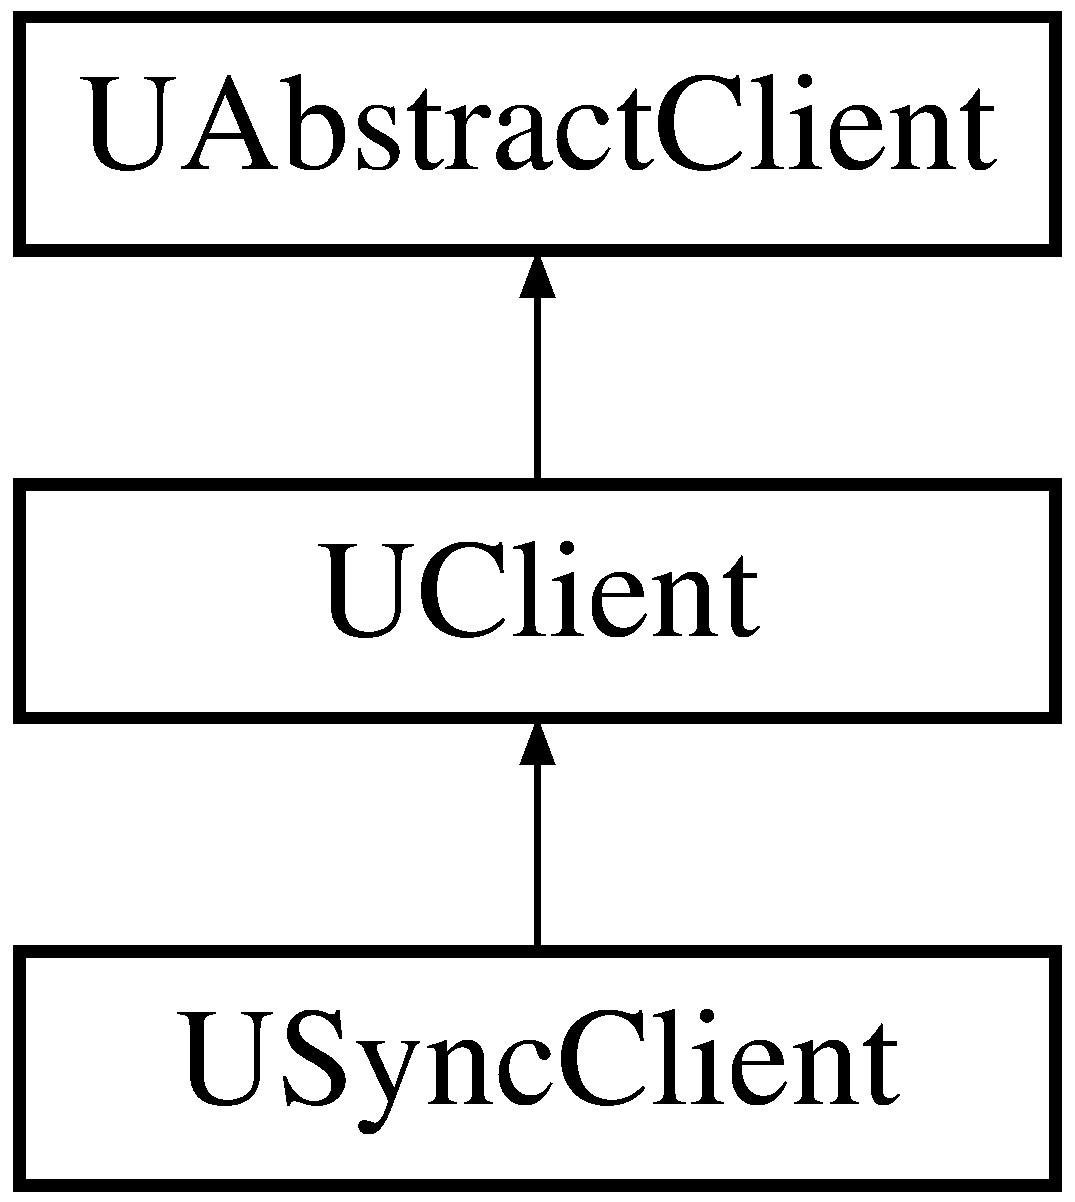
\includegraphics[height=3cm]{classUAbstractClient}
\end{center}
\end{figure}
\subsection*{Public Member Functions}
\begin{CompactItemize}
\item 
{\bf UAbstract\-Client} (const char $\ast$\_\-host, int \_\-port={\bf URBI\_\-PORT}, int \_\-buflen={\bf URBI\_\-BUFLEN})
\begin{CompactList}\small\item\em Create a new instance and connect to the Urbi server. \item\end{CompactList}\item 
int {\bf error} ()\label{classUAbstractClient_a2}

\begin{CompactList}\small\item\em Return current error status, or zero if no error occurred. \item\end{CompactList}\item 
int {\bf send} ()\label{classUAbstractClient_a3}

\begin{CompactList}\small\item\em Function for backward compatibility. Will be removed in future versions. \item\end{CompactList}\item 
int {\bf send} (const char $\ast$format,...)
\begin{CompactList}\small\item\em Send an Urbi command. The syntax is similar to the {\bf printf()}{\rm (p.\,\pageref{classUAbstractClient_a31})} function. \item\end{CompactList}\item 
int {\bf send\-Bin} (const void $\ast$, int len)\label{classUAbstractClient_a5}

\begin{CompactList}\small\item\em Send binary data. \item\end{CompactList}\item 
int {\bf send\-Bin} (const void $\ast$, int len, const char $\ast$header,...)\label{classUAbstractClient_a6}

\begin{CompactList}\small\item\em Send an Urbi header followed by binary data. \item\end{CompactList}\item 
int {\bf start\-Pack} ()
\begin{CompactList}\small\item\em Lock the send buffer (for backward compatibility, will be removed in future versions). \item\end{CompactList}\item 
int {\bf end\-Pack} ()\label{classUAbstractClient_a8}

\begin{CompactList}\small\item\em Unlock the send buffer (for backward compatibility, will be removed in future versions). \item\end{CompactList}\item 
int {\bf pack} (const char $\ast$,...)
\begin{CompactList}\small\item\em Append Urbi commands to the send buffer (for backward compatibility, will be removed in future versions). \item\end{CompactList}\item 
int {\bf vpack} (const char $\ast$, va\_\-list args)\label{classUAbstractClient_a10}

\begin{CompactList}\small\item\em va\_\-list version of pack. \item\end{CompactList}\item 
int {\bf send\-File} (const char $\ast$filename)\label{classUAbstractClient_a11}

\begin{CompactList}\small\item\em Send urbi commands contained in a file. \item\end{CompactList}\item 
UCallback\-ID {\bf send\-Command} ({\bf UCallback}, const char $\ast$,...)\label{classUAbstractClient_a12}

\begin{CompactList}\small\item\em Send a command, prefixing it with a tag, and associate the given callback with this tag. $\ast$/. \item\end{CompactList}\item 
UCallback\-ID {\bf send\-Command} (UCustom\-Callback, void $\ast$, const char $\ast$,...)\label{classUAbstractClient_a13}

\begin{CompactList}\small\item\em Send a command, prefixing it with a tag, and associate the given callback with this tag. $\ast$/. \item\end{CompactList}\item 
int {\bf send\-Sound} (const char $\ast$device, const {\bf USound} \&sound, const char $\ast$tag=0)
\begin{CompactList}\small\item\em Send sound data to the robot for immediate playback. \item\end{CompactList}\item 
int {\bf put\-File} (const char $\ast$local\-Name, const char $\ast$remote\-Name=0)\label{classUAbstractClient_a15}

\begin{CompactList}\small\item\em Put a file on the robot's mass storage device. \item\end{CompactList}\item 
int {\bf put\-File} (const void $\ast$buffer, int length, const char $\ast$remote\-Name)\label{classUAbstractClient_a16}

\begin{CompactList}\small\item\em Save a buffer to a file on the robot. \item\end{CompactList}\item 
UCallback\-ID {\bf set\-Callback} (UCallback\-Wrapper \&callback, const char $\ast$tag)\label{classUAbstractClient_a17}

\begin{CompactList}\small\item\em Associate a callback function with a tag. new style. \item\end{CompactList}\item 
UCallback\-ID {\bf set\-Error\-Callback} (UCallback\-Wrapper \&callback)\label{classUAbstractClient_a18}

\begin{CompactList}\small\item\em Associate a callbaxk function with all error messages. \item\end{CompactList}\item 
UCallback\-ID {\bf set\-Wildcard\-Callback} (UCallback\-Wrapper \&callback)\label{classUAbstractClient_a19}

\begin{CompactList}\small\item\em Associate a callback with all messages. \item\end{CompactList}\item 
UCallback\-ID {\bf set\-Callback} ({\bf UCallback}, const char $\ast$tag)\label{classUAbstractClient_a20}

\begin{CompactList}\small\item\em OLD-style callbacks. \item\end{CompactList}\item 
UCallback\-ID {\bf set\-Callback} (UCustom\-Callback, void $\ast$callback\-Data, const char $\ast$tag)\label{classUAbstractClient_a21}

\begin{CompactList}\small\item\em Associate a callback function with a tag, specifiing a callback custom value that will be passed back to the callback function. \item\end{CompactList}\item 
template$<$class C$>$ UCallback\-ID {\bf set\-Callback} (C \&ref, {\bf UCallback\-Action}(C::$\ast$)(const {\bf UMessage} \&), const char $\ast$tag)\label{classUAbstractClient_a22}

\begin{CompactList}\small\item\em Callback to class member functions(old-style). \item\end{CompactList}\item 
template$<$class C, class P1$>$ UCallback\-ID {\bf set\-Callback} (C \&ref, {\bf UCallback\-Action}(C::$\ast$)(P1, const {\bf UMessage} \&), P1, const char $\ast$tag)\label{classUAbstractClient_a23}

\item 
template$<$class C, class P1, class P2$>$ UCallback\-ID {\bf set\-Callback} (C \&ref, {\bf UCallback\-Action}(C::$\ast$)(P1, P2, const {\bf UMessage} \&), P1, P2, const char $\ast$tag)\label{classUAbstractClient_a24}

\item 
template$<$class C, class P1, class P2, class P3$>$ UCallback\-ID {\bf set\-Callback} (C \&ref, {\bf UCallback\-Action}(C::$\ast$)(P1, P2, P3, const {\bf UMessage} \&), P1, P2, P3, const char $\ast$tag)\label{classUAbstractClient_a25}

\item 
template$<$class C, class P1, class P2, class P3, class P4$>$ UCallback\-ID {\bf set\-Callback} (C \&ref, {\bf UCallback\-Action}(C::$\ast$)(P1, P2, P3, P4, const {\bf UMessage} \&), P1, P2, P3, P4, const char $\ast$tag)\label{classUAbstractClient_a26}

\item 
int {\bf get\-Associated\-Tag} (UCallback\-ID id, char $\ast$tag)
\begin{CompactList}\small\item\em Get the tag associated with a registered callback. \item\end{CompactList}\item 
int {\bf delete\-Callback} (UCallback\-ID call\-Back\-ID)
\begin{CompactList}\small\item\em Delete a callback. \item\end{CompactList}\item 
void {\bf make\-Unique\-Tag} (char $\ast$tag)\label{classUAbstractClient_a29}

\begin{CompactList}\small\item\em Fill tag with a unique tag for this client. \item\end{CompactList}\item 
void {\bf notify\-Callbacks} (const {\bf UMessage} \&msg)
\begin{CompactList}\small\item\em Simulate an Urbi message. \item\end{CompactList}\item 
virtual void {\bf printf} (const char $\ast$format,...)=0\label{classUAbstractClient_a31}

\begin{CompactList}\small\item\em Notify of an error. \item\end{CompactList}\item 
virtual unsigned int {\bf get\-Current\-Time} ()=0\label{classUAbstractClient_a32}

\begin{CompactList}\small\item\em Get time in milliseconds since an unspecified but constant reference time. \item\end{CompactList}\item 
virtual void {\bf lock\-Send} ()=0\label{classUAbstractClient_a33}

\begin{CompactList}\small\item\em Lock the send buffer for exclusive use by the current thread. \item\end{CompactList}\item 
virtual void {\bf unlock\-Send} ()=0\label{classUAbstractClient_a34}

\begin{CompactList}\small\item\em Unlock the send buffer. \item\end{CompactList}\item 
const char $\ast$ {\bf get\-Server\-Name} ()\label{classUAbstractClient_a35}

\begin{CompactList}\small\item\em Return the server name or IP address. \item\end{CompactList}\item 
template$<$class C, class P1$>$ UCallback\-ID {\bf set\-Callback} (C \&ref, {\bf UCallback\-Action}(C::$\ast$func)(P1, const {\bf UMessage} \&), P1 p1, const char $\ast$tag)\label{classUAbstractClient_a36}

\item 
template$<$class C, class P1, class P2$>$ UCallback\-ID {\bf set\-Callback} (C \&ref, {\bf UCallback\-Action}(C::$\ast$func)(P1, P2, const {\bf UMessage} \&), P1 p1, P2 p2, const char $\ast$tag)\label{classUAbstractClient_a37}

\item 
template$<$class C, class P1, class P2, class P3$>$ UCallback\-ID {\bf set\-Callback} (C \&ref, {\bf UCallback\-Action}(C::$\ast$func)(P1, P2, P3, const {\bf UMessage} \&), P1 p1, P2 p2, P3 p3, const char $\ast$tag)\label{classUAbstractClient_a38}

\end{CompactItemize}
\subsection*{Protected Member Functions}
\begin{CompactItemize}
\item 
void {\bf process\-Recv\-Buffer} ()
\begin{CompactList}\small\item\em Called each time new data is available in recv\-Buffer. \item\end{CompactList}\item 
virtual int {\bf effective\-Send} (const void $\ast$buffer, int size)=0\label{classUAbstractClient_b1}

\begin{CompactList}\small\item\em Queue data for sending, returns zero on success, nonzero on failure. \item\end{CompactList}\item 
virtual bool {\bf can\-Send} (int size)=0\label{classUAbstractClient_b2}

\begin{CompactList}\small\item\em Check if successive {\bf effective\-Send()}{\rm (p.\,\pageref{classUAbstractClient_b1})} of cumulated size 'size' will succeed. \item\end{CompactList}\item 
virtual void {\bf lock\-List} ()=0\label{classUAbstractClient_b3}

\begin{CompactList}\small\item\em Lock receive and send portions of the code. \item\end{CompactList}\item 
virtual void {\bf unlock\-List} ()=0\label{classUAbstractClient_b4}

\begin{CompactList}\small\item\em Unlock receive and send portions of the code. \item\end{CompactList}\item 
UCallback\-ID {\bf add\-Callback} (const char $\ast$tag, UCallback\-Wrapper \&w)\label{classUAbstractClient_b5}

\begin{CompactList}\small\item\em Add a callback to the list. \item\end{CompactList}\end{CompactItemize}
\subsection*{Protected Attributes}
\begin{CompactItemize}
\item 
char $\ast$ {\bf host}\label{classUAbstractClient_p0}

\begin{CompactList}\small\item\em Host name. \item\end{CompactList}\item 
int {\bf port}\label{classUAbstractClient_p1}

\begin{CompactList}\small\item\em URBI Port. \item\end{CompactList}\item 
int {\bf buflen}\label{classUAbstractClient_p2}

\begin{CompactList}\small\item\em URBI Buffer length. \item\end{CompactList}\item 
int {\bf rc}\label{classUAbstractClient_p3}

\begin{CompactList}\small\item\em System calls return value storage. \item\end{CompactList}\item 
char $\ast$ {\bf recv\-Buffer}\label{classUAbstractClient_p4}

\begin{CompactList}\small\item\em Reception buffer. \item\end{CompactList}\item 
int {\bf recv\-Buffer\-Position}\label{classUAbstractClient_p5}

\begin{CompactList}\small\item\em Current position in reception buffer. \item\end{CompactList}\end{CompactItemize}
\subsection*{Friends}
\begin{CompactItemize}
\item 
class {\bf UClient\-Streambuf}\label{classUAbstractClient_n0}

\end{CompactItemize}


\subsection{Detailed Description}
Interface for an URBI wrapper object. 

Implementations of this interface are wrappers around the URBI protocol. It handles URBI messages parsing, callback registration and various formatting functions. Implementations of this interface should:\begin{itemize}
\item Redefine error\-Notify() as a function able to notify the user of eventual errors.\item Redfine the four mutual exclusion functions.\item Redefine {\bf effective\-Send()}{\rm (p.\,\pageref{classUAbstractClient_b1})}.\item Fill recv\-Buffer, update recv\-Buffer\-Position and call {\bf process\-Recv\-Buffer()}{\rm (p.\,\pageref{classUAbstractClient_b0})} when new data is available.\item Provide an {\bf execute()}{\rm (p.\,\pageref{namespaceurbi_a5})} function in the namespace urbi, that never returns, and that will be called after initialization.\end{itemize}


See the liburbi-cpp documentation for more informations on how to use this class. 



Definition at line 229 of file uabstractclient.h.

\subsection{Constructor \& Destructor Documentation}
\index{UAbstractClient@{UAbstract\-Client}!UAbstractClient@{UAbstractClient}}
\index{UAbstractClient@{UAbstractClient}!UAbstractClient@{UAbstract\-Client}}
\subsubsection{\setlength{\rightskip}{0pt plus 5cm}UAbstract\-Client::UAbstract\-Client (const char $\ast$ {\em \_\-host}, int {\em \_\-port} = {\tt {\bf URBI\_\-PORT}}, int {\em \_\-buflen} = {\tt {\bf URBI\_\-BUFLEN}})}\label{classUAbstractClient_a0}


Create a new instance and connect to the Urbi server. 

Initializes send\-Buffer and recv\-Buffer, and copy \_\-host and \_\-port. \begin{Desc}
\item[Parameters:]
\begin{description}
\item[{\em \_\-host}]IP address or name of the robot to connect to. \item[{\em \_\-port}]TCP port to connect to. \item[{\em \_\-buflen}]size of send and receive buffers. Implementations should establish the connection in their constructor. \end{description}
\end{Desc}


Definition at line 166 of file uabstractclient.cpp.

References buflen, host, port, rc, and recv\-Buffer.

\subsection{Member Function Documentation}
\index{UAbstractClient@{UAbstract\-Client}!deleteCallback@{deleteCallback}}
\index{deleteCallback@{deleteCallback}!UAbstractClient@{UAbstract\-Client}}
\subsubsection{\setlength{\rightskip}{0pt plus 5cm}int UAbstract\-Client::delete\-Callback (UCallback\-ID {\em callback\-ID})}\label{classUAbstractClient_a28}


Delete a callback. 

Returns 0 if no callback with this id was found, 1 otherwise. 

Definition at line 544 of file uabstractclient.cpp.

References lock\-List(), and unlock\-List().

Referenced by send\-Command(), and send\-Sound().\index{UAbstractClient@{UAbstract\-Client}!getAssociatedTag@{getAssociatedTag}}
\index{getAssociatedTag@{getAssociatedTag}!UAbstractClient@{UAbstract\-Client}}
\subsubsection{\setlength{\rightskip}{0pt plus 5cm}int UAbstract\-Client::get\-Associated\-Tag (UCallback\-ID {\em id}, char $\ast$ {\em tag})}\label{classUAbstractClient_a27}


Get the tag associated with a registered callback. 

Returns 1 and fills tag on success, 0 on failure 

Definition at line 528 of file uabstractclient.cpp.

References lock\-List(), and unlock\-List().\index{UAbstractClient@{UAbstract\-Client}!notifyCallbacks@{notifyCallbacks}}
\index{notifyCallbacks@{notifyCallbacks}!UAbstractClient@{UAbstract\-Client}}
\subsubsection{\setlength{\rightskip}{0pt plus 5cm}void UAbstract\-Client::notify\-Callbacks (const {\bf UMessage} \& {\em msg})}\label{classUAbstractClient_a30}


Simulate an Urbi message. 

Pass the given {\bf UMessage}{\rm (p.\,\pageref{classUMessage})} to all registered callbacks with the corresponding tag, as if it were comming from the URBI server. 

Definition at line 140 of file uabstractclient.cpp.

References lock\-List(), UMessage::tag, UMessage::type, UCallback\-Action, and unlock\-List().

Referenced by process\-Recv\-Buffer().\index{UAbstractClient@{UAbstract\-Client}!pack@{pack}}
\index{pack@{pack}!UAbstractClient@{UAbstract\-Client}}
\subsubsection{\setlength{\rightskip}{0pt plus 5cm}int UAbstract\-Client::pack (const char $\ast$ {\em command},  {\em ...})}\label{classUAbstractClient_a9}


Append Urbi commands to the send buffer (for backward compatibility, will be removed in future versions). 

This function must only be called between a {\bf start\-Pack()}{\rm (p.\,\pageref{classUAbstractClient_a7})} and the corresponding {\bf end\-Pack()}{\rm (p.\,\pageref{classUAbstractClient_a8})}. Data is queued in the send buffer, and sent when {\bf end\-Pack()}{\rm (p.\,\pageref{classUAbstractClient_a8})} is called. 

Definition at line 257 of file uabstractclient.cpp.

References rc, and vpack().\index{UAbstractClient@{UAbstract\-Client}!processRecvBuffer@{processRecvBuffer}}
\index{processRecvBuffer@{processRecvBuffer}!UAbstractClient@{UAbstract\-Client}}
\subsubsection{\setlength{\rightskip}{0pt plus 5cm}void UAbstract\-Client::process\-Recv\-Buffer ()\hspace{0.3cm}{\tt  [protected]}}\label{classUAbstractClient_b0}


Called each time new data is available in recv\-Buffer. 

As long as this function has not returned, neither recv\-Buffer nor recv\-Buffer\-Pos may be modified. 

Definition at line 654 of file uabstractclient.cpp.

References lock\-List(), notify\-Callbacks(), printf(), recv\-Buffer, recv\-Buffer\-Position, and unlock\-List().

Referenced by UClient::listen\-Thread().\index{UAbstractClient@{UAbstract\-Client}!send@{send}}
\index{send@{send}!UAbstractClient@{UAbstract\-Client}}
\subsubsection{\setlength{\rightskip}{0pt plus 5cm}int UAbstract\-Client::send (const char $\ast$ {\em command},  {\em ...})}\label{classUAbstractClient_a4}


Send an Urbi command. The syntax is similar to the {\bf printf()}{\rm (p.\,\pageref{classUAbstractClient_a31})} function. 

Multiple commands can be sent in one call. 

Definition at line 234 of file uabstractclient.cpp.

References effective\-Send(), lock\-Send(), rc, unlock\-Send(), and vpack().\index{UAbstractClient@{UAbstract\-Client}!sendSound@{sendSound}}
\index{sendSound@{sendSound}!UAbstractClient@{UAbstract\-Client}}
\subsubsection{\setlength{\rightskip}{0pt plus 5cm}int UAbstract\-Client::send\-Sound (const char $\ast$ {\em device}, const {\bf USound} \& {\em sound}, const char $\ast$ {\em tag} = {\tt 0})}\label{classUAbstractClient_a14}


Send sound data to the robot for immediate playback. 

If tag is set, an URBI system \char`\"{}stop\char`\"{} message with this tag will be generated when the sound has been played. The sound data is copied in case of asynchronous send, and may be safely deleted as soon as this function returns. 

Definition at line 469 of file uabstractclient.cpp.

References USound::channels, USound::data, delete\-Callback(), make\-Unique\-Tag(), USound::rate, USound::sample\-Format, USound::sample\-Size, send\-Bin(), set\-Callback(), USound::size, and USound::sound\-Format.\index{UAbstractClient@{UAbstract\-Client}!startPack@{startPack}}
\index{startPack@{startPack}!UAbstractClient@{UAbstract\-Client}}
\subsubsection{\setlength{\rightskip}{0pt plus 5cm}int UAbstract\-Client::start\-Pack ()}\label{classUAbstractClient_a7}


Lock the send buffer (for backward compatibility, will be removed in future versions). 

In threaded environnments, this function locks the send buffer so that only the calling thread can call the send functions. Otherwise do nothing. 

Definition at line 215 of file uabstractclient.cpp.

References lock\-Send().

The documentation for this class was generated from the following files:\begin{CompactItemize}
\item 
{\bf uabstractclient.h}\item 
{\bf uabstractclient.cpp}\end{CompactItemize}

\section{UBinary Class Reference}
\label{classUBinary}\index{UBinary@{UBinary}}
Class containing binary data sent by the server, that could not be furtehr interpreted.  


{\tt \#include $<$uabstractclient.h$>$}

\subsection*{Public Attributes}
\begin{CompactItemize}
\item 
void $\ast$ {\bf data}\label{classUBinary_o0}

\begin{CompactList}\small\item\em binary data \item\end{CompactList}\item 
char $\ast$ {\bf message}\label{classUBinary_o1}

\begin{CompactList}\small\item\em message as sent by the server \item\end{CompactList}\item 
int {\bf size}\label{classUBinary_o2}

\end{CompactItemize}


\subsection{Detailed Description}
Class containing binary data sent by the server, that could not be furtehr interpreted. 



Definition at line 126 of file uabstractclient.h.

The documentation for this class was generated from the following file:\begin{CompactItemize}
\item 
{\bf uabstractclient.h}\end{CompactItemize}

\section{UClient Class Reference}
\label{classUClient}\index{UClient@{UClient}}
Linux implementation of {\bf UAbstract\-Client}{\rm (p.\,\pageref{classUAbstractClient})}.  


{\tt \#include $<$uclient.h$>$}

Inheritance diagram for UClient::\begin{figure}[H]
\begin{center}
\leavevmode
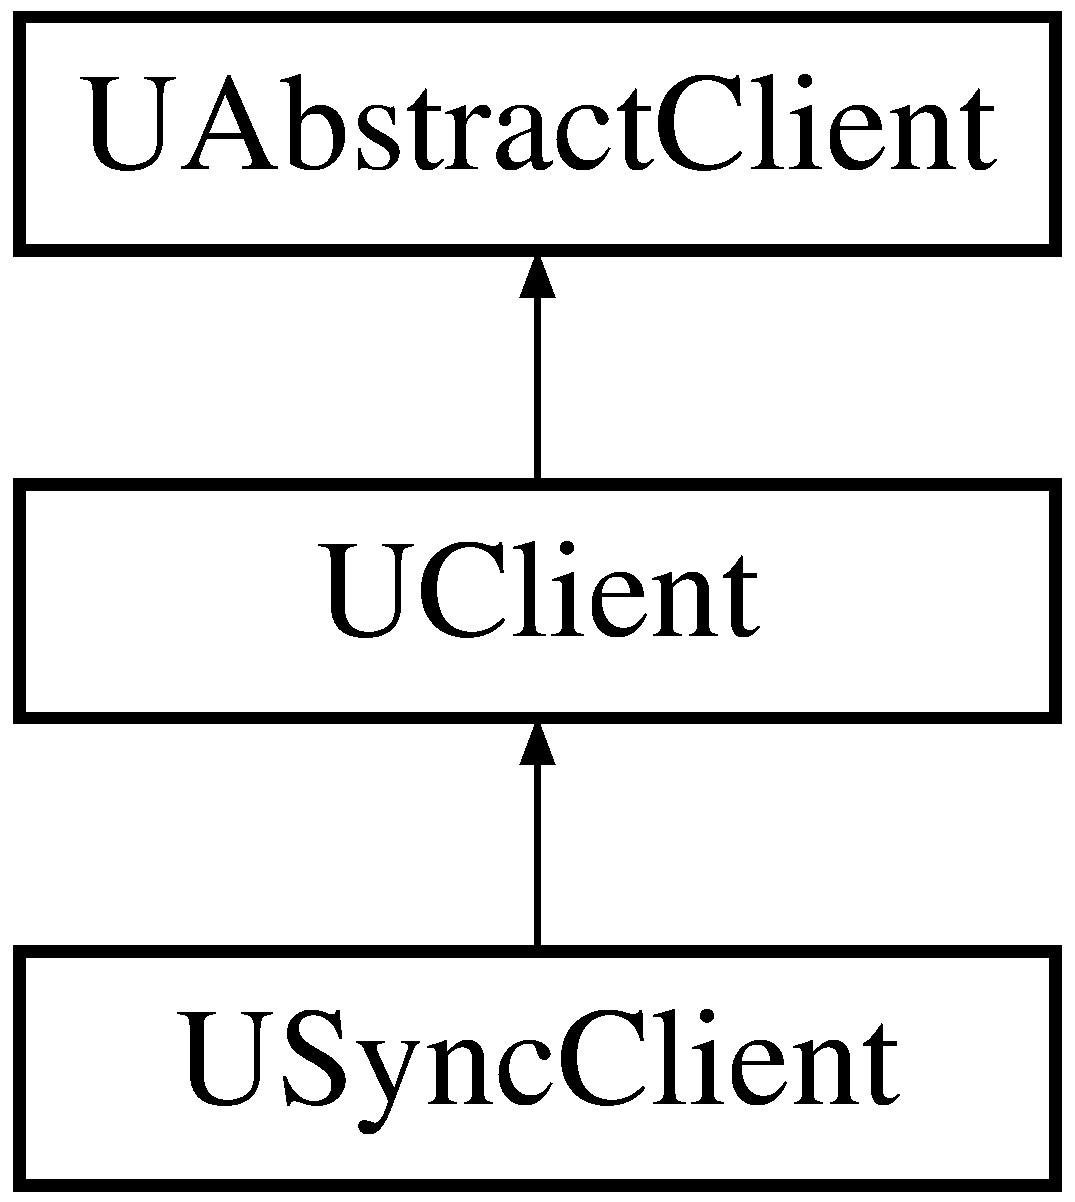
\includegraphics[height=3cm]{classUClient}
\end{center}
\end{figure}
\subsection*{Public Member Functions}
\begin{CompactItemize}
\item 
{\bf UClient} (const char $\ast$\_\-host, int \_\-port={\bf URBI\_\-PORT}, int \_\-buflen={\bf URBI\_\-BUFLEN})
\item 
void {\bf start} ()\label{classUClient_a2}

\begin{CompactList}\small\item\em For compatibility with older versions of the library. \item\end{CompactList}\item 
void {\bf listen\-Thread} ()\label{classUClient_a3}

\begin{CompactList}\small\item\em For internal use. \item\end{CompactList}\item 
virtual void {\bf printf} (const char $\ast$format,...)\label{classUClient_a4}

\begin{CompactList}\small\item\em Notify of an error. \item\end{CompactList}\item 
virtual unsigned int {\bf get\-Current\-Time} ()\label{classUClient_a5}

\begin{CompactList}\small\item\em Get time in milliseconds since an unspecified but constant reference time. \item\end{CompactList}\item 
virtual void {\bf lock\-Send} ()\label{classUClient_a6}

\begin{CompactList}\small\item\em Lock the send buffer for exclusive use by the current thread. \item\end{CompactList}\item 
virtual void {\bf unlock\-Send} ()\label{classUClient_a7}

\begin{CompactList}\small\item\em Unlock the send buffer. \item\end{CompactList}\end{CompactItemize}
\subsection*{Protected Member Functions}
\begin{CompactItemize}
\item 
virtual int {\bf effective\-Send} (const void $\ast$buffer, int size)\label{classUClient_b0}

\begin{CompactList}\small\item\em Queue data for sending, returns zero on success, nonzero on failure. \item\end{CompactList}\item 
virtual bool {\bf can\-Send} (int size)\label{classUClient_b1}

\begin{CompactList}\small\item\em Check if successive {\bf effective\-Send()}{\rm (p.\,\pageref{classUClient_b0})} of cumulated size 'size' will succeed. \item\end{CompactList}\item 
virtual void {\bf lock\-List} ()\label{classUClient_b2}

\begin{CompactList}\small\item\em Lock receive and send portions of the code. \item\end{CompactList}\item 
virtual void {\bf unlock\-List} ()\label{classUClient_b3}

\begin{CompactList}\small\item\em Unlock receive and send portions of the code. \item\end{CompactList}\end{CompactItemize}
\subsection*{Protected Attributes}
\begin{CompactItemize}
\item 
int {\bf sd}\label{classUClient_p0}

\begin{CompactList}\small\item\em Socket file descriptor. \item\end{CompactList}\end{CompactItemize}


\subsection{Detailed Description}
Linux implementation of {\bf UAbstract\-Client}{\rm (p.\,\pageref{classUAbstractClient})}. 

This implementation creates a thread for each instance of UClient, which listens on the associated socket. 



Definition at line 37 of file uclient.h.

\subsection{Constructor \& Destructor Documentation}
\index{UClient@{UClient}!UClient@{UClient}}
\index{UClient@{UClient}!UClient@{UClient}}
\subsubsection{\setlength{\rightskip}{0pt plus 5cm}UClient::UClient (const char $\ast$ {\em \_\-host}, int {\em \_\-port} = {\tt {\bf URBI\_\-PORT}}, int {\em \_\-buflen} = {\tt {\bf URBI\_\-BUFLEN}})}\label{classUClient_a0}


Establish the connection with the server. Spawn a new thread that will listen to the socket, parse the incoming URBI messages, and notify the appropriate callbacks. 

Definition at line 51 of file uclient.cpp.

References urbi::connect(), printf(), and sd.

The documentation for this class was generated from the following files:\begin{CompactItemize}
\item 
{\bf uclient.h}\item 
{\bf uclient.cpp}\end{CompactItemize}

\section{UImage Class Reference}
\label{classUImage}\index{UImage@{UImage}}
Class encapsulating an image.  


{\tt \#include $<$uabstractclient.h$>$}

\subsection*{Public Attributes}
\begin{CompactItemize}
\item 
char $\ast$ {\bf data}\label{classUImage_o0}

\begin{CompactList}\small\item\em pointer to image data \item\end{CompactList}\item 
int {\bf size}\label{classUImage_o1}

\begin{CompactList}\small\item\em image size in byte \item\end{CompactList}\item 
int {\bf width}\label{classUImage_o2}

\item 
int {\bf height}\label{classUImage_o3}

\begin{CompactList}\small\item\em size of the image \item\end{CompactList}\item 
{\bf UImage\-Format} {\bf image\-Format}\label{classUImage_o4}

\end{CompactItemize}


\subsection{Detailed Description}
Class encapsulating an image. 



Definition at line 101 of file uabstractclient.h.

The documentation for this class was generated from the following file:\begin{CompactItemize}
\item 
{\bf uabstractclient.h}\end{CompactItemize}

\section{UMessage Class Reference}
\label{classUMessage}\index{UMessage@{UMessage}}
Class containing all informations related to an URBI message.  


{\tt \#include $<$uabstractclient.h$>$}

\subsection*{Public Member Functions}
\begin{CompactItemize}
\item 
{\bf UMessage} ({\bf UAbstract\-Client} \&{\bf client}, int {\bf timestamp}, char $\ast${\bf tag}, char $\ast${\bf message}, void $\ast$buffer=NULL, int length=0)\label{classUMessage_a0}

\begin{CompactList}\small\item\em This constructor steals the pointers, no copy is made. \item\end{CompactList}\item 
{\bf UMessage} (const {\bf UMessage} \&source, bool alocate=true)\label{classUMessage_a1}

\begin{CompactList}\small\item\em If alocate is true, everything is copied, eles pointers are stolen. \item\end{CompactList}\item 
{\bf $\sim$UMessage} ()\label{classUMessage_a2}

\begin{CompactList}\small\item\em Free everything if data was copied, doesn't free anything otherwise. \item\end{CompactList}\end{CompactItemize}
\subsection*{Public Attributes}
\begin{CompactItemize}
\item 
{\bf UAbstract\-Client} \& {\bf client}\label{classUMessage_o0}

\begin{CompactList}\small\item\em connection from which originated the message \item\end{CompactList}\item 
int {\bf timestamp}\label{classUMessage_o1}

\begin{CompactList}\small\item\em server-side timestamp \item\end{CompactList}\item 
char $\ast$ {\bf tag}\label{classUMessage_o2}

\begin{CompactList}\small\item\em associated tag \item\end{CompactList}\item 
UMessage\-Type {\bf type}\label{classUMessage_o3}

\item 
UBinary\-Message\-Type {\bf binary\-Type}\label{classUMessage_o4}

\item 
double {\bf double\-Value}\label{classUMessage_o5}

\begin{CompactList}\small\item\em float information \item\end{CompactList}\item 
char $\ast$ {\bf string\-Value}\label{classUMessage_o6}

\begin{CompactList}\small\item\em string information \item\end{CompactList}\item 
char $\ast$ {\bf system\-Value}\label{classUMessage_o7}

\begin{CompactList}\small\item\em system information \item\end{CompactList}\item 
char $\ast$ {\bf error\-Value}\label{classUMessage_o8}

\begin{CompactList}\small\item\em error message \item\end{CompactList}\item 
char $\ast$ {\bf message}\label{classUMessage_o9}

\begin{CompactList}\small\item\em unknwon message \item\end{CompactList}\item 
{\bf USound} {\bf sound}\label{classUMessage_o10}

\item 
{\bf UImage} {\bf image}\label{classUMessage_o11}

\item 
{\bf UBinary} {\bf binary}\label{classUMessage_o12}

\end{CompactItemize}


\subsection{Detailed Description}
Class containing all informations related to an URBI message. 



Definition at line 135 of file uabstractclient.h.

The documentation for this class was generated from the following files:\begin{CompactItemize}
\item 
{\bf uabstractclient.h}\item 
{\bf uabstractclient.cpp}\end{CompactItemize}

\section{USound Class Reference}
\label{classUSound}\index{USound@{USound}}
Class encapsulating sound informations.  


{\tt \#include $<$uabstractclient.h$>$}

\subsection*{Public Member Functions}
\begin{CompactItemize}
\item 
bool {\bf operator==} (const {\bf USound} \&b) const \label{classUSound_a0}

\end{CompactItemize}
\subsection*{Public Attributes}
\begin{CompactItemize}
\item 
char $\ast$ {\bf data}\label{classUSound_o0}

\begin{CompactList}\small\item\em pointer to sound data \item\end{CompactList}\item 
int {\bf size}\label{classUSound_o1}

\begin{CompactList}\small\item\em total size in byte \item\end{CompactList}\item 
int {\bf channels}\label{classUSound_o2}

\begin{CompactList}\small\item\em number of audio channels \item\end{CompactList}\item 
int {\bf rate}\label{classUSound_o3}

\begin{CompactList}\small\item\em rate in Hertz \item\end{CompactList}\item 
int {\bf sample\-Size}\label{classUSound_o4}

\begin{CompactList}\small\item\em sample size in bit \item\end{CompactList}\item 
USound\-Format {\bf sound\-Format}\label{classUSound_o5}

\begin{CompactList}\small\item\em format of the sound data \item\end{CompactList}\item 
USound\-Sample\-Format {\bf sample\-Format}\label{classUSound_o6}

\begin{CompactList}\small\item\em sample format \item\end{CompactList}\end{CompactItemize}


\subsection{Detailed Description}
Class encapsulating sound informations. 



Definition at line 110 of file uabstractclient.h.

The documentation for this class was generated from the following file:\begin{CompactItemize}
\item 
{\bf uabstractclient.h}\end{CompactItemize}

\section{USync\-Client Class Reference}
\label{classUSyncClient}\index{USyncClient@{USyncClient}}
{\bf UClient}{\rm (p.\,\pageref{classUClient})} linux implementation with support for synchronous functions.  


{\tt \#include $<$usyncclient.h$>$}

Inheritance diagram for USync\-Client::\begin{figure}[H]
\begin{center}
\leavevmode
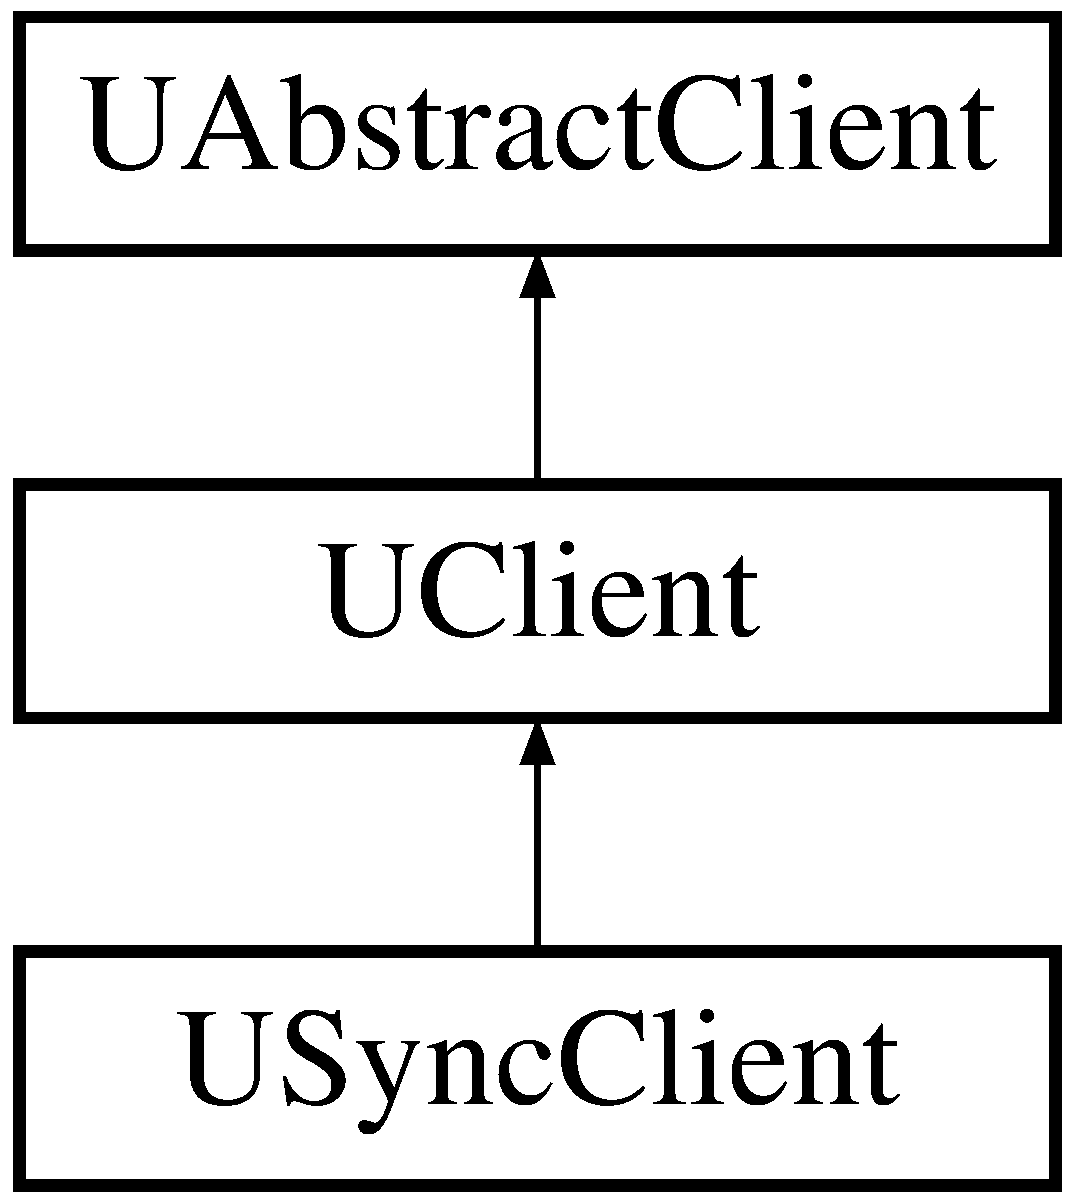
\includegraphics[height=3cm]{classUSyncClient}
\end{center}
\end{figure}
\subsection*{Public Member Functions}
\begin{CompactItemize}
\item 
{\bf USync\-Client} (const char $\ast$\_\-host, int \_\-port={\bf URBI\_\-PORT}, int \_\-buflen={\bf URBI\_\-BUFLEN})\label{classUSyncClient_a0}

\item 
int {\bf sync\-Send} (const void $\ast$buffer, int length)\label{classUSyncClient_a1}

\begin{CompactList}\small\item\em Send given buffer without copying it. \item\end{CompactList}\item 
int {\bf sync\-Get\-Image} (const char $\ast$camera\-Device, void $\ast$buffer, int \&buffersize, int format, int transmit\-Format, int \&width, int \&height)\label{classUSyncClient_a2}

\begin{CompactList}\small\item\em Get an image in a synchronous way. Returns 1 on success, 0 on failure. \item\end{CompactList}\item 
int {\bf sync\-Get\-Device} (const char $\ast$device, double \&val)\label{classUSyncClient_a3}

\begin{CompactList}\small\item\em Get the value of a device in a synchronous way. Returns 1 on success, 0 on failure. \item\end{CompactList}\item 
int {\bf sync\-Get\-Result} (const char $\ast$command, double \&val)\label{classUSyncClient_a4}

\begin{CompactList}\small\item\em Execute an URBI command, return the resulting double value. Returns 1 on success, 0 on failure. \item\end{CompactList}\item 
int {\bf sync\-Get\-Normalized\-Device} (const char $\ast$device, double \&val)\label{classUSyncClient_a5}

\begin{CompactList}\small\item\em Get the normalized value of a device in a synchronous way. Returns 1 on success, 0 on failure. \item\end{CompactList}\item 
int {\bf sync\-Get\-Device} (const char $\ast$device, const char $\ast$field, double \&val)\label{classUSyncClient_a6}

\begin{CompactList}\small\item\em Get a field of a device in a synchronous way. Returns 1 on success, 0 on failure. \item\end{CompactList}\item 
int {\bf sync\-Get\-Sound} (const char $\ast$device, int duration, {\bf USound} \&sound)\label{classUSyncClient_a7}

\begin{CompactList}\small\item\em Get sound for duration milliseconds in buffer. \item\end{CompactList}\end{CompactItemize}


\subsection{Detailed Description}
{\bf UClient}{\rm (p.\,\pageref{classUClient})} linux implementation with support for synchronous functions. 

These functions differs from the {\bf UClient}{\rm (p.\,\pageref{classUClient})} interface in that they are synchronous. One must seriously ponder the fact that they are not easily portable before using them. 



Definition at line 38 of file usyncclient.h.

The documentation for this class was generated from the following files:\begin{CompactItemize}
\item 
{\bf usyncclient.h}\item 
usyncclient.cpp\end{CompactItemize}

\chapter{liburbi-cpp File Documentation}
\section{uabstractclient.cpp File Reference}
\label{uabstractclient_8cpp}\index{uabstractclient.cpp@{uabstractclient.cpp}}
{\tt \#include $<$stdio.h$>$}\par
{\tt \#include $<$stdlib.h$>$}\par
{\tt \#include $<$errno.h$>$}\par
{\tt \#include $<$math.h$>$}\par
{\tt \#include $<$setjmp.h$>$}\par
{\tt \#include $<$algorithm$>$}\par
{\tt \#include $<$sys/stat.h$>$}\par
{\tt \#include \char`\"{}../../lib/jpeg-6b/jpeglib.h\char`\"{}}\par
{\tt \#include \char`\"{}../../lib/jpeg-6b/jerror.h\char`\"{}}\par
{\tt \#include \char`\"{}uabstractclient.h\char`\"{}}\par
\subsection*{Defines}
\begin{CompactItemize}
\item 
\#define {\bf DEBUG}\ 0\label{uabstractclient_8cpp_a0}

\item 
\#define {\bf URBI\_\-ERROR\_\-TAG}\ \char`\"{}[error]\char`\"{}\label{uabstractclient_8cpp_a1}

\item 
\#define {\bf URBI\_\-WILDCARD\_\-TAG}\ \char`\"{}[wildcard]\char`\"{}\label{uabstractclient_8cpp_a2}

\end{CompactItemize}
\subsection*{Enumerations}
\begin{CompactItemize}
\item 
enum {\bf UCallback\-Type} \{ {\bf UCB\_\-}, 
{\bf UCB\_\-C}
 \}
\end{CompactItemize}
\subsection*{Functions}
\begin{CompactItemize}
\item 
void $\ast$ {\bf read\_\-jpeg} (const char $\ast$jpgbuffer, int jpgbuffer\_\-size, bool RGB, int \&output\_\-size)
\item 
{\bf UCallback\-Action} {\bf send\-Sound\_\-} (void $\ast$cb, const {\bf UMessage} \&msg)\label{uabstractclient_8cpp_a7}

\item 
unsigned char {\bf clamp} (float v)\label{uabstractclient_8cpp_a8}

\item 
int {\bf convert\-YCr\-Cbto\-RGB} (const byte $\ast$source\-Image, int buffer\-Size, byte $\ast$destination\-Image)\label{uabstractclient_8cpp_a9}

\item 
int {\bf convert\-JPEGto\-YCr\-Cb} (const byte $\ast$source, int sourcelen, byte $\ast$dest, int \&size)\label{uabstractclient_8cpp_a10}

\item 
int {\bf convert\-JPEGto\-RGB} (const byte $\ast$source, int sourcelen, byte $\ast$dest, int \&size)\label{uabstractclient_8cpp_a11}

\item 
void {\bf init\_\-source} (j\_\-decompress\_\-ptr cinfo)\label{uabstractclient_8cpp_a12}

\item 
boolean {\bf fill\_\-input\_\-buffer} (j\_\-decompress\_\-ptr cinfo)\label{uabstractclient_8cpp_a13}

\item 
void {\bf term\_\-source} (j\_\-decompress\_\-ptr cinfo)\label{uabstractclient_8cpp_a14}

\item 
void {\bf skip\_\-input\_\-data} (j\_\-decompress\_\-ptr cinfo, long num\_\-bytes)\label{uabstractclient_8cpp_a15}

\item 
{\bf urbi\_\-jpeg\_\-error\_\-exit} (j\_\-common\_\-ptr cinfo)\label{uabstractclient_8cpp_a16}

\item 
template$<$class S, class D$>$ void {\bf copy} (S $\ast$src, D $\ast$dst, int sc, int dc, int sr, int dr, int count, bool sf, bool df)\label{uabstractclient_8cpp_a17}

\item 
int {\bf convert} (const {\bf USound} \&source, {\bf USound} \&dest)
\begin{CompactList}\small\item\em Conversion between various sound formats. \item\end{CompactList}\end{CompactItemize}
\subsection*{Variables}
\begin{CompactItemize}
\item 
UCallback\-ID {\bf next\-Id}\label{uabstractclient_8cpp_a3}

\end{CompactItemize}


\subsection{Detailed Description}
\begin{Desc}
\item[Id]{\bf uabstractclient.cpp}{\rm (p.\,\pageref{uabstractclient_8cpp})},v 1.10 2005/05/13 12:13:07 nottale Exp \end{Desc}


Definition of the URBI interface class

Copyright (C) 2004 Jean-Christophe Baillie. All rights reserved.

This program is free software; you can redistribute it and/or modify it under the terms of the GNU General Public License as published by the Free Software Foundation; either version 2 of the License, or (at your option) any later version.

This program is distributed in the hope that it will be useful, but WITHOUT ANY WARRANTY; without even the implied warranty of MERCHANTABILITY or FITNESS FOR A PARTICULAR PURPOSE. See the GNU General Public License for more details.

You should have received a copy of the GNU General Public License along with this program; if not, write to the Free Software Foundation, Inc., 59 Temple Place - Suite 330, Boston, MA 02111-1307, USA.

Definition in file {\bf uabstractclient.cpp}.

\subsection{Function Documentation}
\index{uabstractclient.cpp@{uabstractclient.cpp}!convert@{convert}}
\index{convert@{convert}!uabstractclient.cpp@{uabstractclient.cpp}}
\subsubsection{\setlength{\rightskip}{0pt plus 5cm}int convert (const {\bf USound} \& {\em source}, {\bf USound} \& {\em dest})}\label{uabstractclient_8cpp_a18}


Conversion between various sound formats. 

If any of destination,'s channel, sample\-Size, rate or sample\-Format parameter is 0, values from source will be used. If the desitnation's datasize is too small, data will be realloc()ed, which means one can set data and datasize to zero, and let convert allocate the memory. 

Definition at line 1068 of file uabstractclient.cpp.

References USound::channels, USound::data, USound::rate, USound::sample\-Format, USound::sample\-Size, USound::size, and USound::sound\-Format.

Referenced by USync\-Client::sync\-Get\-Sound().\index{uabstractclient.cpp@{uabstractclient.cpp}!read_jpeg@{read\_\-jpeg}}
\index{read_jpeg@{read\_\-jpeg}!uabstractclient.cpp@{uabstractclient.cpp}}
\subsubsection{\setlength{\rightskip}{0pt plus 5cm}void $\ast$ read\_\-jpeg (const char $\ast$ {\em jpgbuffer}, int {\em jpgbuffer\_\-size}, bool {\em RGB}, int \& {\em output\_\-size})\hspace{0.3cm}{\tt  [static]}}\label{uabstractclient_8cpp_a6}


Convert a jpeg image to YCr\-Cb or RGB. Allocate the buffer with malloc. 

Definition at line 954 of file uabstractclient.cpp.
\section{uabstractclient.h File Reference}
\label{uabstractclient_8h}\index{uabstractclient.h@{uabstractclient.h}}
{\tt \#include $<$stdio.h$>$}\par
{\tt \#include $<$sys/types.h$>$}\par
{\tt \#include $<$string.h$>$}\par
{\tt \#include $<$stdlib.h$>$}\par
{\tt \#include $<$stdarg.h$>$}\par
{\tt \#include $<$list$>$}\par
{\tt \#include $<$iostream$>$}\par
\subsection*{Namespaces}
\begin{CompactItemize}
\item 
namespace {\bf urbi}
\end{CompactItemize}
\subsection*{Classes}
\begin{CompactItemize}
\item 
class {\bf UImage}
\begin{CompactList}\small\item\em Class encapsulating an image. \item\end{CompactList}\item 
class {\bf USound}
\begin{CompactList}\small\item\em Class encapsulating sound informations. \item\end{CompactList}\item 
class {\bf UBinary}
\begin{CompactList}\small\item\em Class containing binary data sent by the server, that could not be furtehr interpreted. \item\end{CompactList}\item 
class {\bf UMessage}
\begin{CompactList}\small\item\em Class containing all informations related to an URBI message. \item\end{CompactList}\item 
class {\bf UAbstract\-Client}
\begin{CompactList}\small\item\em Interface for an URBI wrapper object. \item\end{CompactList}\end{CompactItemize}
\subsection*{Defines}
\begin{CompactItemize}
\item 
\#define {\bf UINVALIDCALLBACKID}\ 0\label{uabstractclient_8h_a0}

\item 
\#define {\bf URBI}(a)\ urbi::unarmor\-And\-Send(\#a)
\begin{CompactList}\small\item\em With this macro, the following code is enough to send a simple command to a robot using URBI: int main() \{ {\bf urbi::connect}{\rm (p.\,\pageref{namespaceurbi_a7})}(\char`\"{}robot\char`\"{}); URBI( head\-Pan.val'n = 0 time:1000 $|$ head\-Tilt.val'n = 0 time:1000, speaker.play(\char`\"{}test.wav\char`\"{}), echo \char`\"{}test\char`\"{}; );. \item\end{CompactList}\end{CompactItemize}
\subsection*{Typedefs}
\begin{CompactItemize}
\item 
typedef unsigned char {\bf byte}\label{uabstractclient_8h_a2}

\item 
typedef unsigned int {\bf UCallback\-ID}\label{uabstractclient_8h_a6}

\item 
typedef {\bf UCallback\-Action}($\ast$ {\bf UCallback} )(const {\bf UMessage} \&msg)\label{uabstractclient_8h_a7}

\begin{CompactList}\small\item\em Callback prototypes. \item\end{CompactList}\item 
typedef {\bf UCallback\-Action}($\ast$ {\bf UCustom\-Callback} )(void $\ast$callback\-Data, const {\bf UMessage} \&msg)\label{uabstractclient_8h_a8}

\end{CompactItemize}
\subsection*{Enumerations}
\begin{CompactItemize}
\item 
enum {\bf UCallback\-Action} \{ {\bf URBI\_\-CONTINUE} = 0, 
{\bf URBI\_\-REMOVE}
 \}
\begin{CompactList}\small\item\em Return values for the callack functions. \item\end{CompactList}\item 
enum {\bf UMessage\-Type} \{ \par
{\bf MESSAGE\_\-DOUBLE}, 
{\bf MESSAGE\_\-STRING}, 
{\bf MESSAGE\_\-BINARY}, 
{\bf MESSAGE\_\-SYSTEM}, 
\par
{\bf MESSAGE\_\-ERROR}, 
{\bf MESSAGE\_\-UNKNOWN}
 \}
\item 
enum {\bf UBinary\-Message\-Type} \{ {\bf BINARYMESSAGE\_\-NONE}, 
{\bf BINARYMESSAGE\_\-UNKNOWN}, 
{\bf BINARYMESSAGE\_\-IMAGE}, 
{\bf BINARYMESSAGE\_\-SOUND}
 \}
\item 
enum {\bf UImage\-Format} \{ {\bf IMAGE\_\-RGB} = 1, 
{\bf IMAGE\_\-YCb\-Cr} = 2, 
{\bf IMAGE\_\-JPEG} = 3, 
{\bf IMAGE\_\-PPM} = 4
 \}
\item 
enum {\bf USound\-Format} \{ {\bf SOUND\_\-RAW}, 
{\bf SOUND\_\-WAV}, 
{\bf SOUND\_\-MP3}, 
{\bf SOUND\_\-OGG}
 \}
\item 
enum {\bf USound\-Sample\-Format} \{ {\bf SAMPLE\_\-SIGNED} = 1, 
{\bf SAMPLE\_\-UNSIGNED} = 2
 \}
\end{CompactItemize}
\subsection*{Functions}
\begin{CompactItemize}
\item 
int {\bf convert\-RGBto\-YCr\-Cb} (const byte $\ast$source, int sourcelen, byte $\ast$dest)\label{uabstractclient_8h_a35}

\begin{CompactList}\small\item\em Image format conversion functions. \item\end{CompactList}\item 
int {\bf convert\-YCr\-Cbto\-RGB} (const byte $\ast$source, int sourcelen, byte $\ast$dest)\label{uabstractclient_8h_a36}

\item 
int {\bf convert\-JPEGto\-YCr\-Cb} (const byte $\ast$source, int sourcelen, byte $\ast$dest, int \&size)\label{uabstractclient_8h_a37}

\item 
int {\bf convert\-JPEGto\-RGB} (const byte $\ast$source, int sourcelen, byte $\ast$dest, int \&size)\label{uabstractclient_8h_a38}

\item 
int {\bf convert} (const {\bf USound} \&source, {\bf USound} \&destination)
\begin{CompactList}\small\item\em Conversion between various sound formats. \item\end{CompactList}\item 
UCallback\-Wrapper \& {\bf callback} ({\bf UCallback} cb)\label{uabstractclient_8h_a40}

\item 
UCallback\-Wrapper \& {\bf callback} (UCustom\-Callback cb, void $\ast$data)\label{uabstractclient_8h_a41}

\item 
template$<$class C$>$ UCallback\-Wrapper \& {\bf callback} (C \&ref, {\bf UCallback\-Action}(C::$\ast$func)(const {\bf UMessage} \&))\label{uabstractclient_8h_a42}

\item 
template$<$class C, class P1$>$ UCallback\-Wrapper \& {\bf callback} (C \&ref, {\bf UCallback\-Action}(C::$\ast$func)(P1, const {\bf UMessage} \&), P1 p1)\label{uabstractclient_8h_a43}

\item 
template$<$class C, class P1, class P2$>$ UCallback\-Wrapper \& {\bf callback} (C \&ref, {\bf UCallback\-Action}(C::$\ast$func)(P1, P2, const {\bf UMessage} \&), P1 p1, P2 p2)\label{uabstractclient_8h_a44}

\item 
template$<$class C, class P1, class P2, class P3$>$ UCallback\-Wrapper \& {\bf callback} (C \&ref, {\bf UCallback\-Action}(C::$\ast$func)(P1, P2, P3, const {\bf UMessage} \&), P1 p1, P2 p2, P3 p3)\label{uabstractclient_8h_a45}

\item 
template$<$class C, class P1, class P2, class P3, class P4$>$ UCallback\-Wrapper \& {\bf callback} (C \&ref, {\bf UCallback\-Action}(C::$\ast$func)(P1, P2, P3, P4, const {\bf UMessage} \&), P1 p1, P2 p2, P3 p3, P4 p4)\label{uabstractclient_8h_a46}

\end{CompactItemize}
\subsection*{Variables}
\begin{CompactItemize}
\item 
const int {\bf URBI\_\-BUFLEN} = 128000\label{uabstractclient_8h_a3}

\begin{CompactList}\small\item\em Connection Buffer size. \item\end{CompactList}\item 
const int {\bf URBI\_\-PORT} = 54000\label{uabstractclient_8h_a4}

\begin{CompactList}\small\item\em Standard port of URBI server. \item\end{CompactList}\item 
const int {\bf URBI\_\-MAX\_\-TAG\_\-LENGTH} = 64\label{uabstractclient_8h_a5}

\begin{CompactList}\small\item\em Maximum length of an URBI tag. \item\end{CompactList}\item 
const char {\bf semicolon} = ';'\label{namespaceurbi_a0}

\item 
const char {\bf pipe} = '$|$'\label{namespaceurbi_a1}

\item 
const char {\bf parallel} = '\&'\label{namespaceurbi_a2}

\item 
const char {\bf comma} = ','\label{namespaceurbi_a3}

\end{CompactItemize}


\subsection{Detailed Description}
\begin{Desc}
\item[Id]{\bf uabstractclient.h}{\rm (p.\,\pageref{uabstractclient_8h})},v 1.7 2005/04/11 13:42:06 nottale Exp \end{Desc}


Definition of the URBI interface class

Copyright (C) 2004 Jean-Christophe Baillie. All rights reserved.

This program is free software; you can redistribute it and/or modify it under the terms of the GNU General Public License as published by the Free Software Foundation; either version 2 of the License, or (at your option) any later version.

This program is distributed in the hope that it will be useful, but WITHOUT ANY WARRANTY; without even the implied warranty of MERCHANTABILITY or FITNESS FOR A PARTICULAR PURPOSE. See the GNU General Public License for more details.

You should have received a copy of the GNU General Public License along with this program; if not, write to the Free Software Foundation, Inc., 59 Temple Place - Suite 330, Boston, MA 02111-1307, USA.

Definition in file {\bf uabstractclient.h}.

\subsection{Define Documentation}
\index{uabstractclient.h@{uabstractclient.h}!URBI@{URBI}}
\index{URBI@{URBI}!uabstractclient.h@{uabstractclient.h}}
\subsubsection{\setlength{\rightskip}{0pt plus 5cm}\#define URBI(a)\ urbi::unarmor\-And\-Send(\#a)}\label{uabstractclient_8h_a1}


With this macro, the following code is enough to send a simple command to a robot using URBI: int main() \{ {\bf urbi::connect}{\rm (p.\,\pageref{namespaceurbi_a7})}(\char`\"{}robot\char`\"{}); URBI( head\-Pan.val'n = 0 time:1000 $|$ head\-Tilt.val'n = 0 time:1000, speaker.play(\char`\"{}test.wav\char`\"{}), echo \char`\"{}test\char`\"{}; );. 

\}

The following construct is also valid: {\bf URBI()}{\rm (p.\,\pageref{uabstractclient_8h_a1})} $<$$<$ \char`\"{}head\-Pan.val=\char`\"{}$<$$<$12$<$$<$\char`\"{};\char`\"{}; 

Definition at line 609 of file uabstractclient.h.

\subsection{Enumeration Type Documentation}
\index{uabstractclient.h@{uabstractclient.h}!UCallbackAction@{UCallbackAction}}
\index{UCallbackAction@{UCallbackAction}!uabstractclient.h@{uabstractclient.h}}
\subsubsection{\setlength{\rightskip}{0pt plus 5cm}enum {\bf UCallback\-Action}}\label{uabstractclient_8h_a47}


Return values for the callack functions. 

Each callback function, when called, must return with either URBI\_\-CONTINUE or URBI\_\-REMOVE:\begin{itemize}
\item URBI\_\-CONTINUE means that the client should continue to call this callbak function.\item URBI\_\-REMOVE means that the client should never call this callback again. \end{itemize}


Definition at line 50 of file uabstractclient.h.

Referenced by UAbstract\-Client::notify\-Callbacks().\index{uabstractclient.h@{uabstractclient.h}!UImageFormat@{UImageFormat}}
\index{UImageFormat@{UImageFormat}!uabstractclient.h@{uabstractclient.h}}
\subsubsection{\setlength{\rightskip}{0pt plus 5cm}enum {\bf UImage\-Format}}\label{uabstractclient_8h_a50}


\begin{Desc}
\item[Enumeration values: ]\par
\begin{description}
\index{IMAGE_RGB@{IMAGE\_\-RGB}!uabstractclient.h@{uabstractclient.h}}\index{uabstractclient.h@{uabstractclient.h}!IMAGE_RGB@{IMAGE\_\-RGB}}\item[{\em 
IMAGE\_\-RGB\label{uabstractclient_8h_a50a25}
}]RGB 24 bit/pixel. \index{IMAGE_YCbCr@{IMAGE\_\-YCbCr}!uabstractclient.h@{uabstractclient.h}}\index{uabstractclient.h@{uabstractclient.h}!IMAGE_YCbCr@{IMAGE\_\-YCbCr}}\item[{\em 
IMAGE\_\-YCb\-Cr\label{uabstractclient_8h_a50a26}
}]YCb\-Cr 24 bit/pixel. \index{IMAGE_JPEG@{IMAGE\_\-JPEG}!uabstractclient.h@{uabstractclient.h}}\index{uabstractclient.h@{uabstractclient.h}!IMAGE_JPEG@{IMAGE\_\-JPEG}}\item[{\em 
IMAGE\_\-JPEG\label{uabstractclient_8h_a50a27}
}]JPEG. \index{IMAGE_PPM@{IMAGE\_\-PPM}!uabstractclient.h@{uabstractclient.h}}\index{uabstractclient.h@{uabstractclient.h}!IMAGE_PPM@{IMAGE\_\-PPM}}\item[{\em 
IMAGE\_\-PPM\label{uabstractclient_8h_a50a28}
}]RGB with a PPM header. \end{description}
\end{Desc}



Definition at line 79 of file uabstractclient.h.

\subsection{Function Documentation}
\index{uabstractclient.h@{uabstractclient.h}!convert@{convert}}
\index{convert@{convert}!uabstractclient.h@{uabstractclient.h}}
\subsubsection{\setlength{\rightskip}{0pt plus 5cm}int convert (const {\bf USound} \& {\em source}, {\bf USound} \& {\em dest})}\label{uabstractclient_8h_a39}


Conversion between various sound formats. 

If any of destination,'s channel, sample\-Size, rate or sample\-Format parameter is 0, values from source will be used. If the desitnation's datasize is too small, data will be realloc()ed, which means one can set data and datasize to zero, and let convert allocate the memory. 

Definition at line 1068 of file uabstractclient.cpp.

References USound::channels, USound::data, USound::rate, USound::sample\-Format, USound::sample\-Size, USound::size, and USound::sound\-Format.

Referenced by USync\-Client::sync\-Get\-Sound().
\section{uclient.cpp File Reference}
\label{uclient_8cpp}\index{uclient.cpp@{uclient.cpp}}
{\tt \#include $<$pthread.h$>$}\par
{\tt \#include $<$stdlib.h$>$}\par
{\tt \#include $<$stdio.h$>$}\par
{\tt \#include $<$errno.h$>$}\par
{\tt \#include $<$sys/time.h$>$}\par
{\tt \#include $<$sys/socket.h$>$}\par
{\tt \#include $<$netinet/in.h$>$}\par
{\tt \#include $<$arpa/inet.h$>$}\par
{\tt \#include $<$netdb.h$>$}\par
{\tt \#include $<$unistd.h$>$}\par
{\tt \#include \char`\"{}uclient.h\char`\"{}}\par
\subsection*{Namespaces}
\begin{CompactItemize}
\item 
namespace {\bf urbi}
\end{CompactItemize}
\subsection*{Functions}
\begin{CompactItemize}
\item 
void $\ast$ {\bf listen\-Thread\-Starter} (void $\ast$object\-Ptr)\label{uclient_8cpp_a1}

\end{CompactItemize}
\subsection*{Variables}
\begin{CompactItemize}
\item 
{\bf UClient} $\ast$ {\bf default\-Client} = 0\label{namespaceurbi_a4}

\end{CompactItemize}


\subsection{Detailed Description}
\begin{Desc}
\item[Id]{\bf uclient.cpp}{\rm (p.\,\pageref{uclient_8cpp})},v 1.7 2005/01/06 11:25:09 nottale Exp \end{Desc}


Linux implementation of the URBI interface class

Copyright (C) 2004 Jean-Christophe Baillie. All rights reserved.

This program is free software; you can redistribute it and/or modify it under the terms of the GNU General Public License as published by the Free Software Foundation; either version 2 of the License, or (at your option) any later version.

This program is distributed in the hope that it will be useful, but WITHOUT ANY WARRANTY; without even the implied warranty of MERCHANTABILITY or FITNESS FOR A PARTICULAR PURPOSE. See the GNU General Public License for more details.

You should have received a copy of the GNU General Public License along with this program; if not, write to the Free Software Foundation, Inc., 59 Temple Place - Suite 330, Boston, MA 02111-1307, USA.

Definition in file {\bf uclient.cpp}.
\section{uclient.h File Reference}
\label{uclient_8h}\index{uclient.h@{uclient.h}}
{\tt \#include \char`\"{}uabstractclient.h\char`\"{}}\par
\subsection*{Namespaces}
\begin{CompactItemize}
\item 
namespace {\bf urbi}
\end{CompactItemize}
\subsection*{Classes}
\begin{CompactItemize}
\item 
class {\bf UClient}
\begin{CompactList}\small\item\em Linux implementation of {\bf UAbstract\-Client}{\rm (p.\,\pageref{classUAbstractClient})}. \item\end{CompactList}\end{CompactItemize}
\subsection*{Functions}
\begin{CompactItemize}
\item 
void {\bf execute} (void)\label{namespaceurbi_a5}

\begin{CompactList}\small\item\em This function must be called at the last line of your main() function. \item\end{CompactList}\item 
void {\bf exit} (int code)\label{namespaceurbi_a6}

\begin{CompactList}\small\item\em This function will terminate your URBI program. \item\end{CompactList}\item 
{\bf UClient} \& {\bf connect} (const char $\ast$host)\label{namespaceurbi_a7}

\begin{CompactList}\small\item\em Creates a new {\bf UClient}{\rm (p.\,\pageref{classUClient})} object. \item\end{CompactList}\item 
{\bf UClient} $\ast$ {\bf get\-Default\-Client} ()\label{namespaceurbi_a8}

\begin{CompactList}\small\item\em Returns the first {\bf UClient}{\rm (p.\,\pageref{classUClient})} created by the program. Used by the URBI macro. \item\end{CompactList}\item 
void {\bf set\-Default\-Client} ({\bf UClient} $\ast$cl)\label{namespaceurbi_a9}

\begin{CompactList}\small\item\em Redefine the default client. \item\end{CompactList}\item 
std::ostream \& {\bf unarmor\-And\-Send} (const char $\ast$str)\label{namespaceurbi_a10}

\begin{CompactList}\small\item\em Send a possibly armored string to the default client. \item\end{CompactList}\end{CompactItemize}


\subsection{Detailed Description}
\begin{Desc}
\item[Id]{\bf uclient.h}{\rm (p.\,\pageref{uclient_8h})},v 1.5 2005/03/17 14:13:09 nottale Exp \end{Desc}


Definition of the URBI interface class

Copyright (C) 2004 Jean-Christophe Baillie. All rights reserved.

This program is free software; you can redistribute it and/or modify it under the terms of the GNU General Public License as published by the Free Software Foundation; either version 2 of the License, or (at your option) any later version.

This program is distributed in the hope that it will be useful, but WITHOUT ANY WARRANTY; without even the implied warranty of MERCHANTABILITY or FITNESS FOR A PARTICULAR PURPOSE. See the GNU General Public License for more details.

You should have received a copy of the GNU General Public License along with this program; if not, write to the Free Software Foundation, Inc., 59 Temple Place - Suite 330, Boston, MA 02111-1307, USA.

Definition in file {\bf uclient.h}.
\section{usyncclient.h File Reference}
\label{usyncclient_8h}\index{usyncclient.h@{usyncclient.h}}
{\tt \#include \char`\"{}uclient.h\char`\"{}}\par
\subsection*{Classes}
\begin{CompactItemize}
\item 
class {\bf USync\-Client}
\begin{CompactList}\small\item\em {\bf UClient}{\rm (p.\,\pageref{classUClient})} linux implementation with support for synchronous functions. \item\end{CompactList}\end{CompactItemize}
\subsection*{Enumerations}
\begin{CompactItemize}
\item 
enum {\bf UTransmit\-Format} \{ {\bf URBI\_\-TRANSMIT\_\-JPEG}, 
{\bf URBI\_\-TRANSMIT\_\-YCb\-Cr}
 \}
\end{CompactItemize}


\subsection{Detailed Description}
\begin{Desc}
\item[Id]{\bf usyncclient.h}{\rm (p.\,\pageref{usyncclient_8h})},v 1.4 2004/12/22 13:06:58 nottale Exp \end{Desc}


Definition of the URBI interface class

Copyright (C) 2004 Jean-Christophe Baillie. All rights reserved.

This program is free software; you can redistribute it and/or modify it under the terms of the GNU General Public License as published by the Free Software Foundation; either version 2 of the License, or (at your option) any later version.

This program is distributed in the hope that it will be useful, but WITHOUT ANY WARRANTY; without even the implied warranty of MERCHANTABILITY or FITNESS FOR A PARTICULAR PURPOSE. See the GNU General Public License for more details.

You should have received a copy of the GNU General Public License along with this program; if not, write to the Free Software Foundation, Inc., 59 Temple Place - Suite 330, Boston, MA 02111-1307, USA.

Definition in file {\bf usyncclient.h}.

\subsection{Enumeration Type Documentation}
\index{usyncclient.h@{usyncclient.h}!UTransmitFormat@{UTransmitFormat}}
\index{UTransmitFormat@{UTransmitFormat}!usyncclient.h@{usyncclient.h}}
\subsubsection{\setlength{\rightskip}{0pt plus 5cm}enum {\bf UTransmit\-Format}}\label{usyncclient_8h_a2}


Format in which image requested with sync\-Get\-Sound are transmitted \begin{Desc}
\item[Enumeration values: ]\par
\begin{description}
\index{URBI_TRANSMIT_JPEG@{URBI\_\-TRANSMIT\_\-JPEG}!usyncclient.h@{usyncclient.h}}\index{usyncclient.h@{usyncclient.h}!URBI_TRANSMIT_JPEG@{URBI\_\-TRANSMIT\_\-JPEG}}\item[{\em 
URBI\_\-TRANSMIT\_\-JPEG\label{usyncclient_8h_a2a0}
}]Transmit images compressed in JPEG. \index{URBI_TRANSMIT_YCbCr@{URBI\_\-TRANSMIT\_\-YCbCr}!usyncclient.h@{usyncclient.h}}\index{usyncclient.h@{usyncclient.h}!URBI_TRANSMIT_YCbCr@{URBI\_\-TRANSMIT\_\-YCbCr}}\item[{\em 
URBI\_\-TRANSMIT\_\-YCb\-Cr\label{usyncclient_8h_a2a1}
}]Transmit raw YCb\-Cr images. \end{description}
\end{Desc}



Definition at line 28 of file usyncclient.h.
\printindex
\end{document}
